% Copyright (c) 2021-2023 Eclipse Arrowhead Project
%
% This program and the accompanying materials are made available under the
% terms of the Eclipse Public License 2.0 which is available at
% http://www.eclipse.org/legal/epl-2.0.
%
% SPDX-License-Identifier: EPL-2.0

\documentclass[a4paper]{arrowhead}

\usepackage[yyyymmdd]{datetime}
\usepackage{enumitem}
\usepackage{etoolbox}
\usepackage[utf8]{inputenc}
\usepackage{multirow}

\renewcommand{\dateseparator}{-}

\begin{document}

%% Arrowhead Document Properties
\ArrowheadTitle{Concepts Reference}
\ArrowheadType{Framework Description}
\ArrowheadTypeShort{FD}
\ArrowheadVersion{0.3}
\ArrowheadDate{\today}
\ArrowheadAuthor{Emanuel Palm and Jerker Delsing}
\ArrowheadOrganization{Eclipse Arrowhead}
\ArrowheadStatus{Proposal}
\ArrowheadContact{emanuel.palm@pinterop.se}
\ArrowheadAbstract{
  This document provides authoritative definitions for the most fundamental concepts of relevance to \textit{Eclipse Arrowhead}, a framework designed to facilitate the effective creation of service-oriented automation systems.
  It is meant to serve as foundation for other documents with relevance to the framework, providing a precise vocabulary untied to any specific practices or technologies.
  It does not contain any architectural patterns or definitions, which means that it, by itself, is not a sufficient foundation for designing Arrowhead systems.
  While its definitions are presented as a model, the document does not endorse any particular modeling language.
}
\ArrowheadFooter{\href{www.arrowhead.eu}{www.arrowhead.eu}}
\ArrowheadSetup
%%

%% Custom Document Commands
\newcommand{\GlossaryHyperRef}[2]{{\color{ArrowheadDarkBlue}\hyperref[sec:glossary:#1]{#2}}}
\newcommand{\GlossaryNameRef}[1]{{\color{ArrowheadDarkBlue}\nameref{sec:glossary:#1}}}
%%

%% Front Page
\ArrowheadFrontPage
%%

%% Table of Contents
\tableofcontents
\newpage
%%

\section{Introduction}
\label{sec:introduction}
% Copyright (c) 2021-10-07 Eclipse Arrowhead Project
%
% This program and the accompanying materials are made available under the
% terms of the Eclipse Public License 2.0 which is available at
% http://www.eclipse.org/legal/epl-2.0.
%
% SPDX-License-Identifier: EPL-2.0

We, the Eclipse Arrowhead project, here present and authoritative set of Arrowhead concept definitions, meant to serve as the foundational language for discussions about and the modelling of Arrowhead-based designs.
The document exists to help mitigate compatibility and consistency issues in software, tooling, models and all other things of relevance to Arrowhead.
The concepts established here are not specified in terms of any particular modelling tools or languages, but should be useful as foundation for any other Arrowhead modelling or documentation effort.

The description of Arrowhead we present here should be seen as an extension of \textit{Reference Architecture Model Industrie 4.0} (RAMI4.0) \cite{adolphs2016reference}.
This means that we take key concepts from RAMI4.0 and present them here in the context of the Arrowhead framework.
As RAMI4.0 is defined partly in terms of \textit{Service-Oriented Architecture} (SOA), we also builds upon \textit{Reference Model for Service Oriented Architecture} (SOA-RM) \cite{mackenzie2006reference}.
In other words, this document assumes a world-view of service-oriented communication in an Industry 4.0 setting.
This world-view is introduced more fully in Section \ref{sec:arrowhead}.

\subsection{Primary Audiences}
\label{sec:introduction:audiences}

This document is being written and maintained with the following primary audiences in mind:

\begin{itemize}
\item \textit{System architects, integrators and developers} designing, integrating or developing Arrowhead systems.
\item \textit{Standardization engineers and researchers} seeking to extend, analyze or improve upon Arrowhead.
\item \textit{Decision makers, users and other stakeholders} that need to understand fundamental Arrowhead concepts.
\end{itemize}

Those seeking a less techincally rigorous description of Arrowhead may want to focus their reading on Section \ref{sec:arrowhead}.
Others are advised to read all sections carefully, in the order they are presented.

\subsection{Scope}
\label{sec:introduction:scope}

We understand a \textit{reference model} to be a set of definitions for technical concepts of fundamental importance to a specific problem domain.
It does not specify how its definitions should be used to design systems, either abstract or concrete.
In the context of this document, the problem domain in question must be understood to be \textit{the design of service-oriented Industry 4.0 systems}.

\GlossaryHyperRef{Reference models}{model-reference} can ve used as vocabularies for defining \GlossaryHyperRef{reference architectures}{architecture-reference}, which in turn can be used to derive \GlossaryHyperRef{concrete architectures}{architecture} and, finally, \GlossaryHyperRef{software implementations}{implementation-software}, as illustrated in Figure \ref{fig:model-implementation-hierarchy}.

\vspace*{\fill}

\begin{figure}[ht]
  \centering
  
\includegraphics{figures/model-implementation-hierarchy}
  \caption{
    The hierarchical levels comprising the steps from reference models to their software implementation, going from highly abstract to entirly concrete.
    Reference models define fundamental concepts, reference architectures adds abstracts limits to how they may be used together, concrete architectures makes those limits realizable in the real world, and implementations do realize all above levels in practice.
  }
  \label{fig:model-implementation-hierarchy}
\end{figure}

\subsection{Notational Conventions}
\label{sec:introduction:conventions}

\subsubsection{Diagrams}

A box with a name inside it denotes a named \GlossaryHyperRef{entity}{entity-model}.
A named arrow between boxes denotes the \GlossaryHyperRef{relation}{relation-model} implied by the name.
If a named arrow has an associated positive integer or range, the relation is to be considered as extending to the number of unique entities indicated by that integer or range.
A range is denoted by $x..y$, where $x$ and $y$ are positive integers and $x<y$.
Omitting $y$ when using the range notation means that the range is infinite from $x$.
A box being inside another box means that it is owned by the containing box.
See Figure \ref{fig:model-implementation-hierarchy} for an example of this graphical notation being used.

Note that this document does \textit{not} define an Arrowhead profile for SysML \cite{omg2019sysml}, or any other modelling language.
The concepts outlined here should corrsepond to the entities and relations defined by any such profiles, however.

\subsubsection{References}

Square brackets around numbers (e.g. \cite{delsing2017iot}) are references to the reference list in Section \ref{sec:references}.
The number within the brackets of any given reference corresponds to the entry with the same number in the reference list.

\subsubsection{Requirements}

Use of the words \textbf{must}, \textbf{must not}, \textbf{required}, \textbf{should}, \textbf{should not}, \textbf{recommended}, \textbf{may}, and \textbf{optional} are to be interpreted as follows when used in this document: \textbf{must} and \textbf{required} denote absolute requirements that must be adhered to for a described entity to be considered as compliant to this reference model; \textbf{must not} denotes an absolute prohibition; \textbf{should}, \textbf{should not} and \textbf{recommended} denote recommendations that should be deviated from only if special circumstances make it relevant; and, finally, \textbf{may} and \textbf{optional} denote something being truly optional.
These word definitions are derived from and are meant to capture what is outlined in RFC 2119 \cite{bradner1997keywords}.

\subsection{Relationships to Other Documents}
\label{sec:introduction:relationships}

The reference model outlined in this document is based on the following works, in order of precedence:

\begin{enumerate}
\item \textit{RAMI4.0} \cite{adolphs2016reference}, which outlines a ontological and architectural view of Industry 4.0.
As RAMI4.0 is a reference \textit{architecture} rather than a reference \textit{model}, however, its 5\textsuperscript{th} section is disregarded and its remaining sections treated as if being a reference model.
This delimitation excludes the ``architectural layers'', ``life-cycle \& value-stream'' phases and ``hierarchical levels'' of RAMI4.0.

\item \textit{SOA-RM} \cite{mackenzie2006reference}, which provides a standardized definition of SOA.
While RAMI4.0 does not include SOA-RM in its reference list, it does mention the standard and requires that all communications adhere to SOA principles. 

\item \textit{Prior work directly concerned with Arrowhead}.
This significantly includes \textit{IoT Automation: Arrowhead Framework} \cite{delsing2017iot}, which was written to provide a comprehensive overview of the framework.

\end{enumerate}

You are not assumed to have read any of the above documents prior to reading this.
Concepts derived from the above sources are reiterated in this document as necessary.

\subsection{Section Overview}
\label{sec:introduction:sections}

\begin{itemize}[leftmargin=3cm,rightmargin=0pt,labelwidth=2cm,labelsep=0pt,itemindent=0pt,parsep=0.1cm,topsep=0.1cm,align=left]

%\item[Section \ref{sec:introduction}]
%This section.

\item[Section \ref{sec:arrowhead}]
An informal overview of Arrowhead, serving both to provide a workable summary of the framework and to prepare readers for better understanding Section \ref{sec:model}.

\item[Section \ref{sec:model}]
The formal and normative description of Arrowhead.

\item[Section \ref{sec:conformance}]
A brief list of requirements, meant to help determine whether or not a given system is conforming to this document.

\item[Section \ref{sec:glossary}]
Lists all significant terms referred to or defined in this document in alphabetical order.

\item[Section \ref{sec:references}]
Lists references to publications referred to in this document.

\item[Section \ref{sec:revision}]
Records the history of changes made to this document.

\end{itemize}


\section{Overview}
\label{sec:overview}
% Copyright (c) 2021-2023 Eclipse Arrowhead Project
%
% This program and the accompanying materials are made available under the
% terms of the Eclipse Public License 2.0 which is available at
% http://www.eclipse.org/legal/epl-2.0.
%
% SPDX-License-Identifier: EPL-2.0

The \GlossaryHyperRef{framework-arrowhead}{Arrowhead framework}, which is illustrated in Figure \ref{fig:framework}, consists of two subframeworks: a \GlossaryHyperRef{framework-idea}{framework of ideas} and a \GlossaryHyperRef{framework-software}{framework of software}.
The framework of ideas formulates and frames the \GlossaryHyperRef{domain-problem}{\textit{problem domain}} the framework of software is meant to help address.
By this we mean that the framework of ideas presents the \GlossaryHyperRef{assumption}{assumptions}, \GlossaryHyperRef{concept}{concepts}, \GlossaryHyperRef{value}{values} and \GlossaryHyperRef{practice}{practices} that should be applied when \GlossaryHyperRef{specification}{specifying} \GlossaryHyperRef{architecture}{architectural} or other technical documentation and when \GlossaryHyperRef{implementation}{implementing} any kinds of Arrowhead systems or components.

\begin{figure}[ht!]
  \centering
  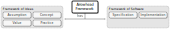
\includegraphics[scale=0.9]{figures/framework}
  \caption{
    The two subframeworks of the Arrowhead framework, concerned with \textit{ideas} and \textit{software}.
    The specifications and implementations of the software framework must conform to the assumptions, concepts, values and practices of the idea framework.
    The concepts of the idea framework are outlined in this document.
  }
  \label{fig:framework}
\end{figure}

This document is part of Arrowhead's framework of ideas.
As such, it is primarily concerned with defining concepts.
However, before we move on to consider our overview those concepts, we will first present a few examples of other key framework ideas.\footnote{
  At the time of writing, the best source of assumptions, values and practices of the Arrowhead framework is Jerker Delsing's book \textit{{IoT} Automation: Arrowhead Framework} \cite{delsing2017iot}.
  The \GlossaryHyperRef{project-eclipse-arrowhead}{Eclipse Arrowhead project} may publish other works of relevance in the future.
}
It is, for example, \textit{assumed} that the framework may be applied in contexts where the primary activity is markedly physical, such as in transportation, mining, manufacturing, electricity generation, healthcare, and so on.
One of the system characteristics \textit{valued} by the framework is \textit{resilience}, or the expectation that every system should do its outmost to mitigate and recover from degradations, failures or other contingencies that may affect its ability to perform its designated tasks.
Finally, one of its \textit{recommended practices} is that every system-of-systems should be thoroughly documented at every level, from its smallest components up to its most high-level interactions.

The rest of this section gives an overview of the most fundamental concepts of the framework.
It is meant to prepare you for the next section, where the same concepts, and other supporting concepts, are presented in greater detail.

\subsection{Stakeholders and Artifacts}

There are two kinds of members of the world of Arrowhead, (1) \GlossaryHyperRef{stakeholder}{stakeholders} and (2) \GlossaryHyperRef{artifact}{artifacts}, as depicted in Figure \ref{fig:world}.
The former denotes a \GlossaryHyperRef{person}{person} or \GlossaryHyperRef{organization}{organization} engaged in an Arrowhead enterprise, while the latter is any thing or object, tangible or intangible, that could be relevant to consider as part of such an enterprise.
Stakeholders \GlossaryHyperRef{owner}{own}, \GlossaryHyperRef{supplier}{supply}, \GlossaryHyperRef{developer}{develop}, \GlossaryHyperRef{operator}{operate}, and \GlossaryHyperRef{user}{use} artifacts, among many other possible activities.
It is their business needs and ambitions that govern what and how Arrowhead artifacts are employed.

\vfill

\begin{figure}[ht!]
  \centering
  
\includegraphics[scale=0.9]{figures/world}
  \caption{
    The two kinds of members of the Arrowhead world: stakeholders and artifacts.
  }
  \label{fig:world}
\end{figure}

\subsection{Devices, Systems and Services}

The most essential types of artifacts in the world of Arrowhead are (1) \GlossaryHyperRef{device}{hardware devices}, (2) \GlossaryHyperRef{system}{software systems} and (3) \GlossaryHyperRef{service}{services}, all shown in Figure \ref{fig:device-system-service}.
\textit{Hardware devices}, or just \textit{devices}, are physical machines, such as servers, robots or tools, that are able to maintain, or \GlossaryHyperRef{hosting-system}{\textit{host}}, \textit{software systems}.
A software system, or just \textit{system}, is a \GlossaryHyperRef{communication}{communicating} \GlossaryHyperRef{instance-software}{software instance} that \GlossaryHyperRef{provision-service}{provides} \textit{services}.
Every service represents a set of tasks a system can perform for other systems or for its stakeholders.
When a system or stakeholder makes use of a service, it is said to \GlossaryHyperRef{consumption-service}{\textit{consume}} it.

\vfill

\begin{figure}[ht!]
  \centering
  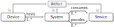
\includegraphics[scale=0.9]{figures/device-system-service}
  \caption{
    Hardware devices \textit{host} software systems, which \textit{consume} and/or \textit{provide} services.
  }
  \label{fig:device-system-service}
\end{figure}

\vfill

Every service represents one area of concern its hosting system can address.
Examples of such areas of concern could be generating financial statements, replacing propellers on drones, manufacturing bolts or measuring humidity.
A service providing control over a door could, for example, make it possible to check if the door is open, to open it and to close it.
Each such activity of every service is represented by one \GlossaryHyperRef{operation}{service operation}, which we will consider more in the next section.

\subsection{Service Provision and Consumption}

As we have already established, \GlossaryHyperRef{communication}{communication} between systems is formulated in terms of the \GlossaryHyperRef{provision-service}{provision} and \GlossaryHyperRef{consumption-service}{consumption} of \GlossaryHyperRef{service}{services}.
\GlossaryHyperRef{system}{Systems} may \textit{provide} services, which other systems can \textit{consume} by sending \GlossaryHyperRef{message}{messages} to their \GlossaryHyperRef{operation}{operations}, as depicted in Figure \ref{fig:service-consumption}.

\vfill

\begin{figure}[ht!]
  \centering
  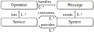
\includegraphics[scale=0.9]{figures/service-consumption}
  \caption{
    Systems consume services by sending messages to the providers of those services.
    Those providers then pass on the messages they receive to their service operations, which interpret and handle them.
  }
  \label{fig:service-consumption}
\end{figure}

\vfill

Also \GlossaryHyperRef{person}{persons} can consume services, even though it is not explicitly depicted in Figure \ref{fig:service-consumption}.
This, however, requires that a \GlossaryHyperRef{interface-human}{human interface} is attached to the providing system, or that another system with such an interface can act as \GlossaryHyperRef{proxy}{proxy}.
The human interface enables the person, via its buttons, prompts or other elements, to send messages to the services in question, just as a regular system would.

When a providing system receives a message from a consuming system or person, it passes it on to the service operation specified in that message, as described in Sections \ref{sec:concepts:service} and \ref{sec:concepts:interface}.
The operation receiving the message will then handle it by performing whatever action it describes, given that the message is \GlossaryHyperRef{message-valid}{valid} and \GlossaryHyperRef{message-permitted}{permitted}.
This handling may entail sending additional messages to other systems, starting or stopping various kinds of automation routines, reading from sensors, electronically signing contracts, sending notifications to an \GlossaryHyperRef{operator}{operator}, sending one or more messages back to the sender, among many other possible examples.

\subsection{System Composition}
\label{sec:overview:system-composition}

\GlossaryHyperRef{system}{Systems} may \GlossaryHyperRef{consumer-service}{consume services} because it is a necessary part of executing the tasks they were designed to perform.
Consider, for example, a scenario in which a number of automated guided vehicles, each of which is a system, are to move items around a factory as directed by a scheduling system.
As the scheduling system does not have wheels, engines or other necessary sensors and actuators, it cannot physically move any items by itself. 
Likewise, the individual vehicles are not capable of themselves deciding what needs to be taken to what location.
However, if the scheduling system may consume the services of the vehicles, it gains the ability to physically execute its plans.
When systems consume each others' services in this manner, they form a \GlossaryHyperRef{system-of-systems}{\textit{system-of-systems}}.

As depicted in Figure \ref{fig:systems-of-systems}, there are different kinds of systems-of-systems with their own characteristics.
There are \GlossaryHyperRef{cloud}{clouds} and \GlossaryHyperRef{system-of-clouds}{systems-of-clouds}, as well as \textit{local} and \textit{virtual} variants of both.\footnote{
  In addition to being local or virtual, a cloud may also be \textit{Arrowhead-compliant}.
  Such a cloud is referred to as an \GlossaryHyperRef{cloud-arrowhead}{\textit{Arrowhead cloud}} and conforms to various architectural requirements put forth by the \GlossaryHyperRef{project-eclipse-arrowhead}{Eclipse Arrowhead project} in a separate document.
}

\vfill

\begin{figure}[ht!]
  \centering
  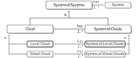
\includegraphics[scale=0.9]{figures/systems-of-systems}
  \caption{
    The types of \textit{systems-of-systems}, each of which consists of a number of \textit{systems} that consume each others' services.
    Clouds are systems-of-systems with \textit{boundaries}, while systems-of-clouds combine multiple clouds.
  }
  \label{fig:systems-of-systems}
\end{figure}

\vfill

A \textbf{cloud} is a set of systems separated from all other systems by at least one \GlossaryHyperRef{boundary-cloud}{boundary}.
Such a boundary may be formed via access control policies, firewalls, gateway systems, physical separation, among many other possible examples.
Additionally, infrastructure must be in place, of any kind, allowing for any system part of the cloud to send messages to any other system in that cloud.\footnote{
  Our term \textit{cloud} must not be confused with \textit{the cloud}, which is a common name for renting virtual compute, storage and networking resources from a so-called \textit{cloud provider}.
}

Because the Arrowhead framework is highly concerned with physical automation processes, we distinguish \GlossaryHyperRef{cloud-local}{local clouds} from \GlossaryHyperRef{cloud-virtual}{virtual clouds}.

A \textbf{local cloud} has at least one system that depends on being at a specific location to provide at least one of its services.
Examples of local clouds could be smelting stations, drone control towers, assembly lines, power distribution centers, or the components of a satellite.
All of these examples involve performing physical activities that depend on occurring at specific physical locations.
Also a common data center may be a local cloud, if its exact location matters for reasons such as privacy or performance.

On the other hand, a \textbf{virtual cloud} has no systems that depend on being at a specific location to provide their services.
In other words, all the \GlossaryHyperRef{resource}{resources} of such a cloud are \GlossaryHyperRef{virtual}{virtual}.
This is the kind of cloud that can be rented by many cloud providers and is part of the greater trend many refer to as \textit{the cloud}.
A virtual cloud could provide services for forecasting, analysis, design, planning or communication, among other possible examples.
None of these use cases require any other resources than virtual compute, storage and network resources.

Individual clouds may be interconnected to former even larger systems-of-systems, which we then refer to as \textbf{systems-of-clouds}.
The individual clouds may be owned and operated by different departments, subdivisions or teams at the same company, or even by different legal entities.
Some of them may be local, while other may be virtual.
Examples of systems-of-clouds may be a set of weather stations operated by the same company, the robots of distinct collaborating companies at a mining site, or the carriers of a supply chain.
When a system-of-clouds contain only local clouds, we refer to it as a \GlossaryHyperRef{system-of-local-clouds}{systems-of-local-clouds}.
Likewise, a system-of-clouds with only virtual clouds constitute a \GlossaryHyperRef{system-of-virtual-clouds}{systems-of-virtual-clouds}.


\section{Concepts}
\label{sec:concepts}
% Copyright (c) 2021 Eclipse Arrowhead Project
%
% This program and the accompanying materials are made available under the
% terms of the Eclipse Public License 2.0 which is available at
% http://www.eclipse.org/legal/epl-2.0.
%
% SPDX-License-Identifier: EPL-2.0

With the major themes of the \GlossaryHyperRef{framework-arrowhead}{Arrowhead framework} now established, we proceed to outline its most significant concepts in detail.
Each subsection of this section \GlossaryHyperRef{description}{describes} one of these concepts, which are as follows:

\vfill

\noindent\begin{tabularx}{\textwidth}{@{} p{0.9cm} p{4.3cm} X @{}}

\ref{sec:concepts:stakeholder} & \textbf{\nameref{sec:concepts:stakeholder}} & A person or \GlossaryHyperRef{organization}{organization} concerned with an \GlossaryHyperRef{entity}{entity} or undertaking. \\
\ref{sec:concepts:entity}      & \textbf{\nameref{sec:concepts:entity}}      & An \GlossaryHyperRef{artifact}{artifact} that can be distinguished from all other artifacts. \\
\ref{sec:concepts:device}      & \textbf{\nameref{sec:concepts:device}}      & A physical \GlossaryHyperRef{entity}{entity} with the \GlossaryHyperRef{capability}{capability} of hosting \GlossaryHyperRef{system}{systems}. \\
\ref{sec:concepts:system}      & \textbf{\nameref{sec:concepts:system}}      & A \GlossaryHyperRef{instance-software}{software instance} able to exercise the \GlossaryHyperRef{capability}{capabilities} of its hosting \GlossaryHyperRef{device}{device}. \\
\ref{sec:concepts:service}     & \textbf{\nameref{sec:concepts:service}}     & A set of \GlossaryHyperRef{operation}{operations} \GlossaryHyperRef{provider-service}{provided} by a \GlossaryHyperRef{system}{system} for other systems to \GlossaryHyperRef{consumer-service}{consume}. \\
\ref{sec:concepts:sos}         & \textbf{\nameref{sec:concepts:sos}}         & A set of \GlossaryHyperRef{system}{systems} that jointly facilitate new \GlossaryHyperRef{capability-system}{capabilities}. \\
\ref{sec:concepts:local-cloud} & \textbf{\nameref{sec:concepts:local-cloud}} & A \GlossaryHyperRef{cloud}{cloud} with a \GlossaryHyperRef{boundary-local}{local boundary} and \GlossaryHyperRef{resource-local}{local resources}.\\
\ref{sec:concepts:solc}        & \textbf{\nameref{sec:concepts:solc}}        & A set of \GlossaryHyperRef{cloud-local}{local clouds} that jointly facilitate new \GlossaryHyperRef{capability-system}{capabilities}.\\
\ref{sec:concepts:network}     & \textbf{\nameref{sec:concepts:network}}     & A set of \GlossaryHyperRef{device}{devices} with \GlossaryHyperRef{interface-network}{network interfaces} that are able to \GlossaryHyperRef{communication}{communicate}.\\
\ref{sec:concepts:interface}   & \textbf{\nameref{sec:concepts:interface}}   & A \GlossaryHyperRef{boundary}{boundary} that can be crossed by the \GlossaryHyperRef{message}{messages} of certain \GlossaryHyperRef{protocol}{protocols}.\\
\ref{sec:concepts:protocol}    & \textbf{\nameref{sec:concepts:protocol}}    & A \GlossaryHyperRef{description}{description} of what \GlossaryHyperRef{message}{messages} can be sent between certain \GlossaryHyperRef{interface}{interfaces}.\\
\ref{sec:concepts:policy}      & \textbf{\nameref{sec:concepts:policy}}      & A set of \GlossaryHyperRef{constraint}{constraints} that must be satisfied for a \GlossaryHyperRef{message}{message} to be \GlossaryHyperRef{message-permitted}{permitted}.\\
\ref{sec:concepts:profile}     & \textbf{\nameref{sec:concepts:profile}}     & A set of \GlossaryHyperRef{constraint}{constraints} added to a \GlossaryHyperRef{protocol}{protocol} or \GlossaryHyperRef{encoding}{encoding}.\\
\ref{sec:concepts:encoding}    & \textbf{\nameref{sec:concepts:encoding}}    & A \GlossaryHyperRef{type-data}{data type} used to formulate and interpret certain \GlossaryHyperRef{message}{messages}.\\
\end{tabularx}

\vspace*{-2mm}

\subsection{Stakeholder}
\label{sec:concepts:stakeholder}

A \GlossaryHyperRef{stakeholder}{stakeholder} is a person or \GlossaryHyperRef{organization}{organization} with \GlossaryHyperRef{stake}{stake} in an \GlossaryHyperRef{entity}{entity} or undertaking with relevance to the \GlossaryHyperRef{framework-arrowhead}{Arrowhead framework}, where \textit{stake} is any form of engagement or commitment.
Stake may be concretely expressed by a stakeholder being associated with one or more \GlossaryHyperRef{role-stakeholder}{\textit{roles}}, as illustrated in Figure \ref{fig:stakeholder}.

\vfill

\begin{figure}[ht!]
  \centering
  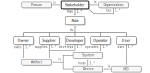
\includegraphics[scale=0.9]{figures/stakeholder}
  \caption{
    The stakeholder as either a person or organization, where each such stakeholder takes on one ore more distinct roles.
    The depicted roles are only possible examples.
    \GlossaryHyperRef{hid}{HID} is an abbreviation for \GlossaryHyperRef{device-human-interface}{Human Interface Device}.
  }
  \label{fig:stakeholder}
\end{figure}

The roles of a given stakeholder dictates what \GlossaryHyperRef{entity}{entities} that person or organization will interact with, as well as the nature of those interactions.
In Figure \ref{fig:stakeholder}, (1) \GlossaryHyperRef{owner}{owner}, (2) \GlossaryHyperRef{supplier}{supplier}, (3) \GlossaryHyperRef{developer}{developer}, (4) \GlossaryHyperRef{operator}{operator} and (5) \GlossaryHyperRef{user}{user} are named explicitly, but more roles are likely to be relevant, such as (6) \GlossaryHyperRef{acquirer}{acquirer} and (7) \GlossaryHyperRef{maintainer}{maintainer}, (8) \GlossaryHyperRef{builder}{builder}, (9) \GlossaryHyperRef{researcher}{researcher} and (10) \GlossaryHyperRef{architect}{architect}.
The listed ten names should be used rather than any synonyms when referring to these particular roles.
Please refer to the \hyperref[sec:glossary]{glossary} for their definitions.
If this document is read electronically, each role name can be clicked to be taken to its definition.

\subsection{Entity}
\label{sec:concepts:entity}

An \GlossaryHyperRef{entity}{entity} is an \GlossaryHyperRef{artifact}{artifact} that it \GlossaryHyperRef{identifiable}{identifiable}, which means that it can be distinguished from all other artifacts.
We use the word \textit{artifact} to refer to any object or thing, physical or intangible.
As depicted in Figure \ref{fig:entity}, this means that an entity always has an \GlossaryHyperRef{identity}{identity}.

\vfill

\begin{figure}[ht!]
  \centering
  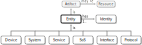
\includegraphics[scale=0.9]{figures/entity}
  \caption{
    The entity as an artifact with an identity.
    An entity or artifact may or may not be considered to be a \GlossaryHyperRef{resource}{resource}, in which case it is deemed to be valuable or useful from the perspective of a \GlossaryHyperRef{stakeholder}{stakeholder}.
    The array of artifacts with an \textit{is}-relation to \textit{Entity} is not complete.
    Other examples include \GlossaryHyperRef{cloud-local}{local clouds}, \GlossaryHyperRef{profile}{profiles} and \GlossaryHyperRef{encoding}{encodings}.
  }
  \label{fig:entity}
\end{figure}

Note that having an identity is not the same as being associated with an \GlossaryHyperRef{identifier}{identifier}, which is a name, number or other value referring to an entity.
It is enough that any such identifier is possible to produce for an artifact to count as an entity.
That being said, certain \GlossaryHyperRef{identification}{identification} requirements, perhaps related to security, performance or discoverability, may make it impractical to treat any other artifacts as entities than those with identifiers.

\subsection{Device}
\label{sec:concepts:device}

A \GlossaryHyperRef{device}{device} is a physical \GlossaryHyperRef{entity}{entity} with certain automation and compute \GlossaryHyperRef{capability-device}{capabilities}.
Examples of capabilities include moving robotic arms, reading from sensors, running \GlossaryHyperRef{software}{software} and sending \GlossaryHyperRef{message}{messages}.
Every device must be capable of \GlossaryHyperRef{hosting-system}{\textit{hosting}} at least one \GlossaryHyperRef{system}{system}, which are \GlossaryHyperRef{communication}{communicating} \GlossaryHyperRef{instance-software}{software instances}.
Devices consist of \GlossaryHyperRef{component-hardware}{hardware components}.
While there are no limits to what such components can make up a device, each device must always have (1) \GlossaryHyperRef{unit-memory}{memory}, (2) \GlossaryHyperRef{unit-compute}{compute} and (3) \GlossaryHyperRef{interface-network}{network interfacing} components, as shown in Figure \ref{fig:device}.

\vfill

\begin{figure}[ht!]
  \centering
  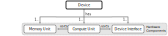
\includegraphics[scale=0.9]{figures/device}
  \caption{
    The device as a set of hardware components, each with automation or compute capabilities.
    Every device must be able to host software components using its compute and memory units, as well as communicate with other devices via its network interfaces.
    Devices with \GlossaryHyperRef{interface-human}{human interfaces} are able to communicate directly with \GlossaryHyperRef{person}{persons}.
    Other examples of hardware components could be sensors, actuators, compute accelerators and batteries.
  }
  \label{fig:device}
\end{figure}

Every device must be able to host at least one system, or it is to be considered as being a hardware component.
While it may seem unintuitive to consider certain machines as components, such as large pumping complexes or vehicles with only manual controls, the \GlossaryHyperRef{framework-arrowhead}{Arrowhead framework} is meant to facilitate automation through the use of interconnected devices with compute capabilities.
If a machine cannot run software, making it able to host systems, that capability must be added before it can play a meaningful role in an \GlossaryHyperRef{arrowhead}{Arrowhead} context.
Consequently, machines without system hosting capabilities must either be considered as components or not be considered from the perspective of Arrowhead at all.

\newpage

\subsection{System}
\label{sec:concepts:system}

A \GlossaryHyperRef{system}{system} is an \GlossaryHyperRef{identifiable}{identifiable} \GlossaryHyperRef{instance-software}{software instance} that is \GlossaryHyperRef{hosting-system}{hosted} by a \GlossaryHyperRef{device}{device}.
As shown in Figure \ref{fig:system}, a system consists of \GlossaryHyperRef{component-software}{software components}.
Just as \GlossaryHyperRef{component-hardware}{hardware components}, software components can have various types of automation or compute \GlossaryHyperRef{capability-system}{capabilities}.
Every system should have the capability of \GlossaryHyperRef{consumer-service}{consuming services}, \GlossaryHyperRef{provider-service}{providing services}, or both.
If a given system can do neither, it must be referred to as an \GlossaryHyperRef{system-opaque}{\textit{opaque system}}.

\vfill

\begin{figure}[ht!]
  \centering
  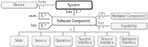
\includegraphics[scale=0.9]{figures/system}
  \caption{
    The system as a set of related software components, endowing a hosting device with new automation or compute capabilities.
    Other examples of software components could be operating systems, files, file systems, software libraries, programming language runtimes, databases and virtual machines.
  }
  \label{fig:system}
\end{figure}

Note that systems are not required to have any particular relationships to operating system processes, binary formats, virtual machines, and so on.
They may be \GlossaryHyperRef{implementation-software}{implemented} in any way deemed suitable.

\subsection{Service}
\label{sec:concepts:service}

A \GlossaryHyperRef{service}{service} is an \GlossaryHyperRef{identifiable}{identifiable} set of \GlossaryHyperRef{interface-service}{service interfaces} and \GlossaryHyperRef{operation-service}{operations}.
Each \textit{service interface} had by a service represents one way in which is can receive \GlossaryHyperRef{message}{messages}, while each of its \textit{operations} represents one activity the \GlossaryHyperRef{system}{system} \GlossaryHyperRef{provider-service}{providing} the service can perform, if a \GlossaryHyperRef{message-valid}{valid} and \GlossaryHyperRef{message-permitted}{permitted} message is received.
As depicted in Figure \ref{fig:service}, service interfaces pass on, or \GlossaryHyperRef{routing-message}{\textit{route}}, received messages to \GlossaryHyperRef{interface-operation}{operation interfaces}, each of which may execute one operation with a message as argument.
Those operations may send additional messages via the same or other operation interfaces, which will pass them on toward other operations as described in Section \ref{sec:concepts:interface}.

\vfill

\begin{figure}[ht!]
  \centering
  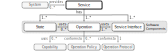
\includegraphics[scale=0.9]{figures/service}
  \caption{
    The service as a set of service interfaces and operations, making it possible for a providing system to offer the use of its capabilities to consuming systems via its service interfaces.
  }
  \label{fig:service}
\end{figure}

As all operations are \GlossaryHyperRef{component-software}{software components}, they may use any \GlossaryHyperRef{capability}{capabilities} of the devices and systems that host and provide them, respectively.
Once successfully consumed, an operation may send any number of messages to service operations provided by other systems, with any kinds of delays or intervals.
When a service starts up and shuts down, it may be considered as if receiving an implicit message via an \textit{initialize} or \textit{terminate} operation, respectively.
The messages to both of these operations may carry \GlossaryHyperRef{configuration}{configuration} \GlossaryHyperRef{data}{data} produced by and/or given to the system providing the service.
It should not be possible for other systems to consume the initialize and terminate operations while the service in question is being provided.

\subsection{System-of-Systems}
\label{sec:concepts:sos}

A \GlossaryHyperRef{system-of-systems}{system-of-systems} is a set of at least two \GlossaryHyperRef{system}{systems}, together facilitating one or more \GlossaryHyperRef{capability-system}{capabilities} none of the constituent systems could have on its own.
The facilitation of new capabilities is accomplished by the systems providing services and/or consuming each other's services.

While it may seem as if consuming services would hardly be enough for new capabilities to always emerge, it actually is the case.
For example, let us assume that a system has the capability of turning on and off a light.
That system also provides a service allowing for other systems to request that the light be turned on or off.
If a different system can successfully consume that service, it also gains the capability of turning on and off that particular light.
As a new system now may control that particular light, a new capability has emerged.

\subsection{Local Cloud}
\label{sec:concepts:local-cloud}

A \GlossaryHyperRef{cloud-local}{local cloud} is an \GlossaryHyperRef{identifiable}{identifiable} \GlossaryHyperRef{system-of-systems}{system-of-systems} able to execute given tasks through the use of a pool of \GlossaryHyperRef{resource}{resources}.
The resource pool of a local cloud could contain 3D-printers, autonomous unmanned vehicles, conventional servers, or anything else producing a value on demand.
As depicted in Figure \ref{fig:local-cloud}, the local cloud is distinct from other types of \GlossaryHyperRef{cloud}{clouds} by having at least one \GlossaryHyperRef{boundary-local}{local boundary} and one \GlossaryHyperRef{resource-local}{local resource}, which means that it is physically tied to a concrete location.
A local cloud could be engaged in manufacturing, repairs, heating, electricity distribution, workspace monitoring, drone fleet control, among many other possible kinds of physical activities.
A local cloud may be stationary or mobile.
A cloud that has no resources or boundaries tied to any particular physical locations should be referred to as a \GlossaryHyperRef{cloud-virtual}{\textit{virtual cloud}}.

\vfill

\begin{figure}[ht!]
  \centering
  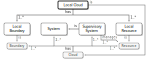
\includegraphics[scale=0.9]{figures/local-cloud}
  \caption{
    The local cloud as a regular cloud with at least one local boundary and one local resource.
  }
  \label{fig:local-cloud}
\end{figure}

That a local cloud has a boundary means that a distinction is being made between \GlossaryHyperRef{system}{systems} inside and outside the cloud.
A boundary being local means that the distinction is being made by a physical \GlossaryHyperRef{attribute}{attribute}, such as device location, type of device, or physical attachment to a certain \GlossaryHyperRef{entity}{entity}.
Boundaries may be protected, which means that measures are in place to guarantee security, safety, real-time characteristics, or other local cloud attributes.
The resources of a local cloud may be of any type, from virtual compute resources to physical drills or pumps.
A system managing a resource may be referred to as a \GlossaryHyperRef{system-supervisory}{\textit{supervisory system}}.

\subsection{System-of-Local-Clouds}
\label{sec:concepts:solc}

A \GlossaryHyperRef{system-of-local-clouds}{system-of-local-clouds} is two or more \GlossaryHyperRef{cloud-local}{local clouds} that \GlossaryHyperRef{consumer-service}{consume} each other's \GlossaryHyperRef{service}{services} to facilitate new \GlossaryHyperRef{capability-system}{capabilities}.
It is similar to the local cloud, with the exception of its \GlossaryHyperRef{subsystem}{subsystems} are \GlossaryHyperRef{cloud-local}{local clouds} instead of plain \GlossaryHyperRef{system}{systems}.
A system-of-local-clouds may have its own \GlossaryHyperRef{boundary-cloud}{boundaries} in addition to those of its constituent local clouds.
Those boundaries are formed by attributes shared by all the constituent local clouds, such as certificates issued by the same organization, or physical attachment to the same network bus.
A system-of-local-clouds cannot have resources beyond those of its constituent clouds, however.

\subsection{Network}
\label{sec:concepts:network}

A \GlossaryHyperRef{network}{network} is a set of two or more \GlossaryHyperRef{device}{devices}, \GlossaryHyperRef{connection}{connected} via \GlossaryHyperRef{interface-network}{network interfaces} such that \GlossaryHyperRef{message}{messages} can pass between them.
As shown in Figure \ref{fig:network}, devices may be \GlossaryHyperRef{interconnection}{interconnected} via \GlossaryHyperRef{device-intermediary}{intermediary devices}, examples of which could be routers, switches, hubs, busses and firewalls.
The term \GlossaryHyperRef{device-end}{\textit{end device}} may be used to represent any device not being an intermediary device.
Any technology able to connect devices is treated as facilitating networks, even if not typically associated with conventional networking methods.

\vfill

\begin{figure}[ht!]
  \centering
  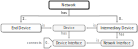
\includegraphics[scale=0.9]{figures/network}
  \caption{
    The network as a set of connected end devices, potentially interconnected via intermediary devices.
  }
  \label{fig:network}
\end{figure}

\vspace*{-6mm}

\subsection{Interface}
\label{sec:concepts:interface}

An \GlossaryHyperRef{interface}{interface} is an \GlossaryHyperRef{identifiable}{identifiable} \GlossaryHyperRef{boundary}{boundary} over which \GlossaryHyperRef{message}{messages} adhering to a supported \GlossaryHyperRef{protocol}{protocol} can cross, if those messages also satisfy all \GlossaryHyperRef{policy}{policies} associated with that interface.
When considering \GlossaryHyperRef{service}{service} \GlossaryHyperRef{provision-service}{provision} and \GlossaryHyperRef{consumption-service}{consumption}, four types of interfaces become particularly relevant.
These are (1) \GlossaryHyperRef{interface-network}{network interfaces}, (2) \GlossaryHyperRef{interface-system}{system interfaces}, (3) \GlossaryHyperRef{interface-service}{service interfaces} and (4) \GlossaryHyperRef{interface-operation}{operation interfaces}, arranged as outlined in Figure \ref{fig:interface}.

\vfill

\begin{figure}[ht!]
  \centering
  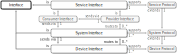
\includegraphics[scale=0.9]{figures/interface}
  \caption{
    The interface as a set of supported protocols and enforced policies.
    Devices, systems, services and operations have their own interface types, forming four stages through which messages can be passed.
  }
  \label{fig:interface}
\end{figure}

These four interface types form four stages, beginning with the network interface to the left and ending with the operation interface to the right.
When a network interface receives a message, it is \GlossaryHyperRef{routing-message}{\textit{routed}} rightwards through each stage until it is found to be \GlossaryHyperRef{message-invalid}{invalid}, \GlossaryHyperRef{message-forbidden}{forbidden} or reaches an \GlossaryHyperRef{operation-service}{operation}.
If the message is found to be invalid or forbidden, an \GlossaryHyperRef{message-error}{error message} may be propagated back to its sender.
The receiving operation may react by sending additional messages, each of which will then be \textit{sent} leftwards until it reaches a network interface.
The network interface will send the message via \GlossaryHyperRef{network}{networks} until it reaches a device interface, which will repeat the receiving procedure we just covered.
The operation first sending the message should be notified of any errors, both those received as messages and those noticed through other means.

Each interface only supports a single protocol and can only pass on messages of that protocol.
For it to be possible to pass messages between stages, the protocol of the left stage must be \textit{extended} by the protocol of the right stage.
If, for example, a network interface supports the IP protocol \cite{deering2017internet} and system interface the TCP/IP \cite{postel1981transmission} protocol, messages can pass between the two as the latter protocol is an extension of the former.
The interface at each stage may elect to base its routing decision on any protocol details, including those used by earlier stages.
This means that all three of the network, system and service stages may base their routing decisions on IP addresses, for example, if relevant to whatever use case is being targeted.

\subsection{Protocol}
\label{sec:concepts:protocol}

A \GlossaryHyperRef{protocol}{protocol} is an \GlossaryHyperRef{identifiable}{identifiable} set of \GlossaryHyperRef{type-message}{message} and \GlossaryHyperRef{type-state}{state} types, useful for determining what \GlossaryHyperRef{message}{messages} may move through the \GlossaryHyperRef{interface}{interfaces} that support them.
\textit{Message types} determine what \GlossaryHyperRef{data}{data} conformant messages must and may contain, while each \textit{state type} dictates when certain messages are acceptable in relation to a certain \GlossaryHyperRef{state-protocol}{state}.
As shown in Figure \ref{fig:protocol}, a protocol may also be defined as an \GlossaryHyperRef{protocol-extensible}{extension} of another protocol, conform to certain \GlossaryHyperRef{profile-protocol}{profiles} and use certain \GlossaryHyperRef{encoding}{encodings}.
Profiles and encodings are described in Sections \ref{sec:concepts:profile} and \ref{sec:concepts:encoding}.

\vfill

\begin{figure}[ht!]
  \centering
  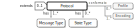
\includegraphics[scale=0.9]{figures/protocol}
  \caption{
    The protocol as set of message and state types, conforming to certain profiles.
  }
  \label{fig:protocol}
\end{figure}

A protocol may, when relevant, be considered as a \GlossaryHyperRef{function}{function} useful for testing if a given message is \GlossaryHyperRef{message-valid}{valid} or \GlossaryHyperRef{message-invalid}{invalid} with respect to a current state.
If the message is valid, the function returns the type of the message, which is needed to interpret the contents of that message.
If the message is invalid, the function returns an indication of why the message failed to satisfy the message and/or state types of the protocol. 

Protocols should only be concerned with the \textit{destination} and \textit{interpretation} of messages, not with whether they are \GlossaryHyperRef{message-permitted}{\textit{permitted}} or not.
This means that states should be associated with protocols only to ensure that received messages can be passed on or understood correctly.
If, for example, a service controlling a door receives an message telling it to open its already open door, what does the sender of the message expect to happen?
Nothing at all?
That it closes and opens again?
This ambiguity can be avoided by having the protocol be aware of the state of the door.
Messages received when their interpretation is unclear can then be rejected.

\subsection{Policy}
\label{sec:concepts:policy}

A \GlossaryHyperRef{policy}{policy} is an \GlossaryHyperRef{identifiable}{identifiable} set of \GlossaryHyperRef{constraint-policy}{constraints}, useful for determining if given \GlossaryHyperRef{message}{messages} are \GlossaryHyperRef{message-permitted}{permitted} or \GlossaryHyperRef{message-forbidden}{forbidden}, as depicted in Figure \ref{fig:policy}.
Policies may be concerned with authorization, contracts, economic goals, and so on.

\vfill

\begin{figure}[ht!]
  \centering
  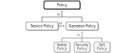
\includegraphics[scale=0.9]{figures/policy}
  \caption{
    The policy as a set of constraints, useful for determining if messages are permitted or not.
  }
  \label{fig:policy}
\end{figure}

Every policy may, when relevant, be regarded as a \GlossaryHyperRef{function-predicate}{predicate function} useful for testing if given message is permitted with respect to any kind of information.
Policies are typically enforced by \GlossaryHyperRef{interface}{interfaces}, as described in Section \ref{sec:concepts:interface}.
If a \GlossaryHyperRef{message}{message} is forbidden with respect to one or more of the policies of an interface, those policies should be listed in any error message returned to the sender of that message.

While \GlossaryHyperRef{protocol}{protocols} help determine if a given message can be passed on or interpreted correctly, \textit{policies} are meant to determine if the activity described by that message would occur under desirable conditions.
For example, an interface may receive a message requesting that a certain pump be started.
While the interpretation of the message may be clear, there may still be other conditions that make it undesirable for the pump to activate.
If the pump is on fire, turning it on may present a safety hazard; if the system attempting to start the pump is unauthorized, the risk is higher for sabotage and other wasteful behaviors; and so on.

\newpage

\subsection{Profile}
\label{sec:concepts:profile}

A \textit{profile} is a set of \GlossaryHyperRef{constraint}{constraints} that can be added to a \GlossaryHyperRef{protocol}{protocol}.
While a protocol may only extend up to one other protocol, it may conform to any number of profiles.
In Figure \ref{fig:profile}, two significant types of constraints are illustrated, the \GlossaryHyperRef{constraint-protocol}{protocol constraint} and the \GlossaryHyperRef{constraint-encoding}{encoding constraint}.

\begin{figure}[ht!]
  \centering
  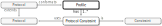
\includegraphics[scale=0.9]{figures/profile}
  \caption{
    The profile as a set of constraints, which may, for example, be concerned with protocols or encodings.
  }
  \label{fig:profile}
\end{figure}

A \textit{protocol constraint} is defined in terms of a protocol that must be extended by any protocols conforming to its owning profile. 
For example, a \GlossaryHyperRef{interface-service}{service interface} may support a custom extension of the HTTP protocol \cite{fielding2014hypertext}.
Such an extended HTTP protocol would, among other things, specify how a message will be routed from a system interface to a service interface, as described in Section \ref{sec:concepts:interface}.
If that custom protocol is meant to be conformant to a certain profile, the constraints of that profile must be formulated in terms of HTTP without the extension, or any other protocol HTTP extends, namely TCP/IP \cite{postel1981transmission} or IP \cite{deering2017internet}.
The profile in question may require that certain HTTP headers be included in every message, that certain TCP flags not be used, and so on.
A protocol constraint could specify how authorization tokens are to be included in certain messages, for example.

An \textit{encoding constraint} is defined in terms of an \GlossaryHyperRef{encoding}{encoding} that must be used by any protocols conforming to its owning profile.
Such a constraint could be used to force message payloads to adhere to a certain semantics, such as SenML \cite{rfc8428}.

\subsection{Encoding}
\label{sec:concepts:encoding}

An \textit{encoding} is ...

%As a special case, a lone encoding, such as JSON \cite{rfc7159}, can be considered as being a protocol without any states or messages.
%This enables a profile to be concerned only with \GlossaryHyperRef{message-type}{message types}, perhaps useful as message payloads.

%\textit{Encodings} introduce \GlossaryHyperRef{system-type}{type systems} in which message data can be expressed.
%If a protocol defines its messages without referring to an encoding, it is considered to have a \textit{custom} encoding.

\begin{figure}[ht!]
  \centering
  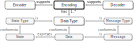
\includegraphics[scale=0.9]{figures/encoding}
  \caption{
    The encoding as set of data types, supported by certain encoders and decoders.
  }
  \label{fig:encoding}
\end{figure}

\section{Conformance Requirements}
\label{sec:conformance}
% Copyright (c) 2021 Eclipse Arrowhead Project
%
% This program and the accompanying materials are made available under the
% terms of the Eclipse Public License 2.0 which is available at
% http://www.eclipse.org/legal/epl-2.0.
%
% SPDX-License-Identifier: EPL-2.0

TODO

A list of requirements that must be satisfied in order for a document to be considered conformant to this documentation reference.

\section{Glossary}
\label{sec:glossary}
% Copyright (c) 2021-10-07 Eclipse Arrowhead Project
%
% This program and the accompanying materials are made available under the
% terms of the Eclipse Public License 2.0 which is available at
% http://www.eclipse.org/legal/epl-2.0.
%
% SPDX-License-Identifier: EPL-2.0

{

\newcommand{\GlossaryEntry}[2]{\paragraph{#1}\label{sec:glossary:#2}\,}
\newcommand{\GlossaryNote}[2]{\begin{minipage}[b]{\dimexpr\linewidth-0.5cm\relax}\vspace*{0.33cm}\footnotesize{\textbf{#1}\ #2}\end{minipage}}

\GlossaryEntry{Abstract}{abstract}
See \GlossaryNameRef{model-abstract}

\GlossaryEntry{Administration}{administration}

\GlossaryEntry{Administrator}{administrator}

\GlossaryEntry{ANI}{ani}
See \GlossaryNameRef{interface-application-network}.

\GlossaryEntry{API}{api}
See \GlossaryNameRef{interface-application-programming}.

\GlossaryEntry{Application}{application}

\GlossaryEntry{Architecture}{architecture}
A \GlossaryHyperRef{concrete model}{model-concrete} of a \GlossaryHyperRef{system-of-systems}{system-of-systems} defined in terms of certain \GlossaryHyperRef{reference models}{model-reference}, \GlossaryHyperRef{reference architectures}{architecture-reference}, \GlossaryHyperRef{protocols}{protocol}, \GlossaryHyperRef{profiles}{profile} and \GlossaryHyperRef{specifications}{specification}.
See also Section \ref{sec:introduction:scope}.

	\GlossaryNote{Note 1}{
		An \GlossaryHyperRef{architecture}{architecture} can be extended by another architecture or realized as a concrete system-of-systems.
	}

	\GlossaryNote{RAMI4.0}{
	    defines architecture as the ``combination of elements of a model based on principles and rules for constructing, refining and using it''.
		We consider ``combinations of elements of a model'' to be a ``model of a system-of-systems'' and to be ``based on principles and rules for constructing, refining and using it'' as building upon the artifacts we list above.
		Our definition should be interpreted as being compatible but more specific.
	}

	\GlossaryNote{SOA-RM}{
		defines software architecture as ``the structure or structures of an information system consisting of entities and their externally visible properties, and the relationships among them''.
		That definition is equivalent to our definition of \GlossaryHyperRef{model}{model}, with the exception that the thing being modelled has to be an information system.
		As our definition is concerned with a model and a system-of-systems, which must be an information system, we regard out definition as compatible but more specific.
	}

\GlossaryEntry{Architecture, Reference}{architecture-reference}
An \GlossaryHyperRef{abstract model}{model-abstract} of a \GlossaryHyperRef{system-of-systems}{system-of-systems} defined in terms of certain \GlossaryHyperRef{reference models}{model-reference}, abstract \GlossaryHyperRef{protocols}{protocol}, abstract \GlossaryHyperRef{profiles}{profile} and abstract \GlossaryHyperRef{specifications}{specification}.

	\GlossaryNote{Note 1}{
		A reference architecture can be extended by another reference architecture or be \GlossaryHyperRef{concretized}{concretization-model} by a regular \GlossaryHyperRef{architecture}{architecture}.
	}

	\GlossaryNote{RAMI4.0}{
		defines reference architecture as a ``model for an architecture description (for I[ndustry ]4.0) which is generally used and recognized as being suitable (has reference character)''.
		We consider ``model for an architecture description'' to be a ``model of a system-of-systems'' and assume that there is no need to explicitly mention that a given reference architecture must be suitable for meeting real-world business objectives or be useful as foundation for other architectures.
		ur definition should be interpreted as being compatible but more specific.
	}

	\GlossaryNote{SOA-RM}{
	    defines reference architecture as ``an architectural design pattern that indicates how an abstract set of mechanisms and relationships realizes a predetermined set of requirements''.
	    It complements its definition with explanations in its first section, which also make it clear that a reference architecture is defined in terms of \GlossaryHyperRef{protocols}{protocol}, \GlossaryHyperRef{profiles}{profile}, \GlossaryHyperRef{specifications}{specification} and standards, the latter of which we understand to be any other the earlier three in standardized form.
	    While we let the part about requirements be implicit, our definition should be interpreted as being compatible but more specific.
	}

\GlossaryEntry{Arrowhead}{arrowhead}

\GlossaryEntry{Asset}{asset}
An object, tangible or intangible, that is of value to an \GlossaryHyperRef{organization}{organization}.

	\GlossaryNote{RAMI4.0}{
		defines asset as an ``object which has a value for an organization''.
		Our definition should be interpreted as being equivalent.
	}

\GlossaryEntry{Authentication}{authentication}

\GlossaryEntry{Authorization}{authorization}

\GlossaryEntry{Capability}{capability}
An action that can be performed by a \GlossaryHyperRef{service provider}{provider-service}.

	\GlossaryNote{SOA-RM}{
		defines a capability as ``a real-world effect that a service provider is able to provide to a service consumer''.
		To stress that a ``real-world effect'' also could be related to a purely digital event, such as data being sent or altered, we replace the term with ``action''.
		Our definition should be interpreted as being equivalent.
	}

\GlossaryEntry{Certificate}{certificate}

\GlossaryEntry{Cloud}{cloud}

\GlossaryEntry{Cloud, Compute}{cloud-compute}

\GlossaryEntry{Cloud, Local}{cloud-local}

\GlossaryEntry{Cloud, Storage}{cloud-storage}

\GlossaryEntry{Cloud, Virtual}{cloud-virtual}

\GlossaryEntry{Codec}{codec}
%A \GlossaryHyperRef{model}{model} specifying a fundamental set of \GlossaryHyperRef{primitive}{type-primitive} and \GlossaryHyperRef{structured}{type-structured} \GlossaryHyperRef{data}{data} \GlossaryHyperRef{types}{type-data} useful for \GlossaryHyperRef{coding}{coding} data.
%A codec can be either \GlossaryHyperRef{abstract}{codec-abstract} or \GlossaryHyperRef{concrete}{codec-concrete}.

%\GlossaryEntry{Codec, Abstract}{codec-abstract}
%A \GlossaryHyperRef{codec}{codec} specified only in terms of \GlossaryHyperRef{abstract data types}{type-abstract-data}.
%Such a codec can be used to \GlossaryHyperRef{model}{model} \GlossaryHyperRef{abstract messages}{message-abstract}, serve as \GlossaryHyperRef{component}{component} of a larger abstract codec, or \GlossaryHyperRef{constrain}{constraint-model} a \GlossaryHyperRef{concrete codec}{codec-concrete}.

%\GlossaryEntry{Codec, Concrete}{codec-concrete}
%A \GlossaryHyperRef{codec}{codec} specified only in terms of \GlossaryHyperRef{concrete data types}{type-concrete-data}.
%Such a codec can be used to \GlossaryHyperRef{encode}{encoding} and \GlossaryHyperRef{decode}{decoding} \GlossaryHyperRef{concrete messages}{message-concrete}, or serve as \GlossaryHyperRef{component}{component} of a larger concrete codec.

\GlossaryEntry{Coding}{coding}
Transforming \GlossaryHyperRef{data}{data} from being expressed in one \GlossaryHyperRef{codec}{codec} into another.
See also \GlossaryHyperRef{decoding}{decoding} and \GlossaryHyperRef{encoding}{encoding}.

\GlossaryEntry{Coding, A}{coding-a}
Synonymous to \GlossaryNameRef{codec}.

\GlossaryEntry{Component}{component}
A part of a \GlossaryHyperRef{system}{system}, contributing to it facilitating its \GlossaryHyperRef{capabilities}{capability}.

	\GlossaryNote{Note 1}{
		While it is also correct that a system can be regarded as a component of a \GlossaryHyperRef{system-of-systems}{system-of-systems}, we associate the word ``component'' primarily with plain systems.
		When referring to the systems of a system-of-systems, we recommend using the words ``system'' and ``subsystem'' to avoid confusion.
	}

	\GlossaryNote{Note 2}{
		A component is practically distinct from a system by being unable to \GlossaryHyperRef{provide}{provider-service} or \GlossaryHyperRef{consume}{consumer-service} \GlossaryHyperRef{services}{service} independently.
	}

\GlossaryEntry{Concrete}{concrete}
See \GlossaryNameRef{model-concrete}.

\GlossaryEntry{Concretization, Model}{concretization-model}
Making an \GlossaryHyperRef{abstract model}{model-abstract} less abstract by \GlossaryHyperRef{specifying}{specification} details required to realize it.

\GlossaryEntry{Configuration}{configuration}

\GlossaryEntry{Constraint, Model}{constraint-model}
A \GlossaryHyperRef{model relation}{relation} where one \GlossaryHyperRef{entity}{entity-model} imposes constraints, or limits, on the other.

	\GlossaryNote{Note 1}{
		The presence of explicit model constraints enable \GlossaryHyperRef{model validation}{validation-model}.
	}

	\GlossaryNote{Note 2}{
		Perhaps a bit counterintuitively, a constraint \textit{adds} information to the constrained entity by narrowing down the the ways in which it could be realized.
		See also \GlossaryNameRef{property-model} and \GlossaryNameRef{specification}.
	}

\GlossaryEntry{Consumer, Service}{consumer-service}
A \GlossaryHyperRef{system}{system} currently \GlossaryHyperRef{invoking}{invocation-function} a \GlossaryHyperRef{function}{function} \GlossaryHyperRef{provided}{provider-service} via a \GlossaryHyperRef{service}{service}.

	\GlossaryNote{SOA-RM}{
		defines a service consumer as ``an entity which seeks to satisfy a particular need through the use [of] capabilities offered by means of a service''.
		We require that the one consuming the service is (1) a \GlossaryHyperRef{system}{system} rather than just any \GlossaryHyperRef{entity}{entity}, (2) that the \GlossaryHyperRef{capabilities}{capability} of the consumed service be exercised by invoking a function, as well as (3) that the invocation satisfies a service consumption policy.
	}

%\GlossaryEntry{Context}{context}
%A \GlossaryHyperRef{model}{model} of an \GlossaryHyperRef{abstract}{context-abstract} or \GlossaryHyperRef{concrete}{context-concrete} environment in which a \GlossaryHyperRef{model entity}{entity-model} can be situated.
%The entity in question is \GlossaryHyperRef{constrained}{constraint-model} by, or limited to, the \GlossaryHyperRef{data}{data} and other resources the context provides.

%\GlossaryEntry{Context, Abstract}{context-abstract}
%A \GlossaryHyperRef{model}{model} of an abstract environment in which an abstract \GlossaryHyperRef{entity}{entity} can be situated.
%It can serve as \GlossaryHyperRef{reference}{model-reference} for or \GlossaryHyperRef{component}{component} of another \GlossaryHyperRef{context}{context}, or as a \GlossaryHyperRef{constraint}{constraint-model} for an \GlossaryHyperRef{abstract architecture}{architecture-abstract}.

%\GlossaryEntry{Context, Concrete}{context-concrete}
%A \GlossaryHyperRef{model}{model} of a concrete environment in which a concrete \GlossaryHyperRef{entity}{entity} can be situated.
%It can serve as \GlossaryHyperRef{reference}{model-reference} for or \GlossaryHyperRef{component}{component} of another \GlossaryHyperRef{concrete context}{context-concrete}, or as a \GlossaryHyperRef{constraint}{constraint-model} for a \GlossaryHyperRef{concrete architecture}{architecture-concrete}.

\GlossaryEntry{Data}{data}
A sequence of datums, such as binary digits or other symbols, expressing a set of \GlossaryHyperRef{descriptions}{description}.

	\GlossaryNote{Note 1}{
		The descriptions can only be interpreted if the \GlossaryHyperRef{data types}{type-data} used to organize the datums are known to the interpreter.
	}

\GlossaryEntry{Decoding}{decoding}
The process through which \GlossaryHyperRef{data}{data} is transformed from being expressed in a \GlossaryHyperRef{codec}{codec} suitable for transmission or storage to another codec suitable for interpretation.

	\GlossaryNote{Note 1}{
		The operation is the reverse of \GlossaryHyperRef{encoding}{encoding}.
	}

	\GlossaryNote{Note 2}{
		The term can also be used to express the act of a human interpreting data.
	}


\GlossaryEntry{Description}{description}
\GlossaryHyperRef{Data}{data} about a \GlossaryHyperRef{entity}{entity}, concretely represented by a \GlossaryHyperRef{model}{model}, a human-readable text, or both.

\GlossaryEntry{Description, Interface Design}{description-interface-design}

\GlossaryEntry{Design}{design}

\GlossaryEntry{Design, Interface}{design-interface}

\GlossaryEntry{Device}{device}

\GlossaryEntry{Device, Human Interface (HID)}{device-human-interface}

\GlossaryEntry{Encoding}{encoding}
The process through which \GlossaryHyperRef{data}{data} is transformed from being expressed in a \GlossaryHyperRef{codec}{codec} suitable for interpretation to another codec suitable for transmission or storage.

	\GlossaryNote{Note 1}{
		The operation is the reverse of \GlossaryHyperRef{decoding}{decoding}.
	}

	\GlossaryNote{Note 2}{
		The term can also be used to express the act of a human recording data.
	}

\GlossaryEntry{Encoding, An}{encoding-an}
Synonymous to \GlossaryNameRef{codec}.

\GlossaryEntry{Entity}{entity}
An object, tangible or intangible, that is uniquely \GlossaryHyperRef{identifiable}{identity}.

	\GlossaryNote{Note 1}{
		An entity being uniquely identifiable does not necessarily mean that it is associated with a \GlossaryHyperRef{certificate}{certificate} or \GlossaryHyperRef{identifier}{identifier}.
		It only means that a \GlossaryHyperRef{description}{description} can be rendered that unambigously refers to the entity in question.
	}

	\GlossaryNote{RAMI4.0}{
		defines entity as an ``uniquely identifiable object which is administered in the information world due to its importance''.
		Our definition should be interpreted as being equivalent.
	}

	\GlossaryNote{SOA-RM}{
	    mentions the word ``entity'' nine times, but provides no explicit definition.
	    We assume their definition to match that of a regular English dictionary, such as ``something that has separate and distinct existence and objective or conceptual reality'' \cite{webster2021entity}.
		Our definition should be interpreted as being equivalent.
	}

\GlossaryEntry{Entity, Model}{entity-model}
An \GlossaryHyperRef{entity}{entity} represented as part of a \GlossaryHyperRef{model}{model}.

\GlossaryEntry{Framework}{framework}

\GlossaryEntry{Function}{function}
An \GlossaryHyperRef{invocable}{invocation-function} \GlossaryHyperRef{subroutine}{subroutine} adhering to the \GlossaryHyperRef{protocol}{protocol} established by a certain \GlossaryHyperRef{signature}{signature-functon}.

\GlossaryEntry{HID}{hid} See \GlossaryNameRef{device-human-interface}.

\GlossaryEntry{Industry 4.0}{industry40}

\GlossaryEntry{Identification}{identification}
The process through which an \GlossaryHyperRef{entity}{entity} collects and verifies the \GlossaryHyperRef{identity}{identity} of another entity. 

\GlossaryEntry{Identifier}{identifier}
\GlossaryHyperRef{Data}{data} associated with an \GlossaryHyperRef{entity}{entity} that allows for it to be \GlossaryHyperRef{identified}{identification}.

\GlossaryEntry{Identity}{identity}
The aspect or aspects, such as \GlossaryHyperRef{identifiers}{identifier}, that makes an \GlossaryHyperRef{entity}{entity} distinct from all other entities.

\GlossaryEntry{Interface}{interface}

\GlossaryEntry{Interface, Administrative}{interface-administrative}

\GlossaryEntry{Interface, Application Network (ANI)}{interface-application-network}

\GlossaryEntry{Interface, Application Programming (API)}{interface-application-programming}

\GlossaryEntry{Interface, Management}{interface-management}

\GlossaryEntry{Interface, Network}{interface-network}

\GlossaryEntry{Interface, Operator}{interface-operator}

\GlossaryEntry{Invocation, Function}{invocation-function}
The attempt to trigger the \GlossaryHyperRef{capabilities}{capability} associated with a \GlossaryHyperRef{function}{function} by sending a \GlossaryHyperRef{message}{message} to the \GlossaryHyperRef{service}{service} through which the function is \GlossaryHyperRef{provided}{provider-service}.
See also \GlossaryNameRef{signature-function}. TODO: Make use of subroutine definition to simplify this.

\GlossaryEntry{Manager}{manager}

\GlossaryEntry{Management}{management}

\GlossaryEntry{Message}{message}

\GlossaryEntry{Metadata}{metadata}

\GlossaryEntry{Model}{model}
A representation of facts in the form of a graph, consisting of \GlossaryHyperRef{entities}{entity-model}, \GlossaryHyperRef{relations}{relation-model} and \GlossaryHyperRef{properties}{property-model}.
Models can be expressed as visual diagrams, text or binary data.
They can be human-readable, machine-readable, or both.
They can be either \GlossaryHyperRef{abstract}{model-abstract} or \GlossaryHyperRef{concrete}{model-concrete}.
See also \GlossaryNameRef{model-reference}.

\GlossaryEntry{Model, Abstract}{model-abstract}
A \GlossaryHyperRef{model}{model} that is insufficiently specified to be possible to realize as a concrete artifact.
Abstract models can be used for imposing \GlossaryHyperRef{constraints}{constraint-model} on other models, which creates room for producing \GlossaryHyperRef{reference arhictecures}{architecture-reference}, abstract \GlossaryHyperRef{service descriptions}{service}, and so on.

\GlossaryEntry{Model, Concrete}{model-concrete}
A \GlossaryHyperRef{model}{model} that is sufficiently specified to be possible to realize as a concrete artifact, such as a \GlossaryHyperRef{protocol}{protocol} or \GlossaryHyperRef{software}{software}.

\GlossaryEntry{Model, Reference}{model-reference}
An \GlossaryHyperRef{abstract model}{model-abstract} defining technical concepts of fundamental importance to a specific problem domain.
See also Section \ref{sec:introduction:scope}.

	\GlossaryNote{RAMI4.0}{
		defines reference model as a ``model that is generally used and recognized as being suitable (has recommendation character) for deriving
specific models.
		We adds that the model must be abstract and define fundamental concepts for a problem domain, setting it apart as more significant than other abstract models.
	}

	\GlossaryNote{SOA-RM}{
		defines reference model as ``an abstract framework for understanding significant relationships among the entities of some environment that enables the development of specific architectures using consistent standards or specifications supporting that environment''.
		It further clarifies that a ``reference model consists of a minimal set of unifying concepts, axioms and relationships within a particular problem domain, and is independent of specific standards, technologies, implementations, or other concrete details''.
		Our definition should be interpreted as being equivalent.
	}

\GlossaryEntry{Model, Specific}{model-specific}
See \GlossaryNameRef{model-concrete}.

\GlossaryEntry{Operator}{operator}

\GlossaryEntry{Organization}{organization}

\GlossaryEntry{Policy}{policy}

\GlossaryEntry{Policy, Service Consumption}{policy-service-consumption}

\GlossaryEntry{Process, Application}{process-application}

\GlossaryEntry{Profile}{profile}
A \GlossaryHyperRef{model}{model} imposing constraints on a \GlossaryHyperRef{protocol}{protocol}.
A profile could specify a \GlossaryHyperRef{protocol stack}{stack-protocol}, certain message semantics, how authentication and authorization are to be carried out, among many other possible examples.

\GlossaryEntry{Property, Model}{property-model}
Named \GlossaryHyperRef{data}{data} associated with either a model \GlossaryHyperRef{entity}{entity-model} or \GlossaryHyperRef{relation}{relation-model}.

\GlossaryEntry{Protocol}{protocol}
A \GlossaryHyperRef{model}{model} of communication defined in terms of \GlossaryHyperRef{messages}{message}.
See also \GlossaryNameRef{stack-protocol}.

\GlossaryEntry{Provider, Service}{provider-service}
A \GlossaryHyperRef{system}{system} that makes \GlossaryHyperRef{services}{service} available for \GlossaryHyperRef{consumption}{consumer-service} by any systems able to satisfy its \GlossaryHyperRef{consumption policies}{policy-service-consumption}.

	\GlossaryNote{SOA-RM}{
		defines a service provider as ``an entity (person or organization) that offers the use of capabilities by means of a service''.
		Our definition is more specific in that it requires the \GlossaryHyperRef{entity}{entity} be a system.
	}

\GlossaryEntry{Relation, Model}{relation-model}
A uni-directional association of two \GlossaryHyperRef{entities}{entity-model} part of the same \GlossaryHyperRef{model}{model}.

\GlossaryEntry{Service}{service}
A set of \GlossaryHyperRef{functions}{function} that can be \GlossaryHyperRef{provided}{provider-service} via an \GlossaryHyperRef{interface}{interface}.

	\GlossaryNote{RAMI4.0}{
		defines a service as ``separate scope of functions offered by an entity or organization via interfaces''.
		Our definition restricts service provision to systems.
	}

	\GlossaryNote{SOA-RM}{
		defines a service as ``the means by which the needs of a consumer are brought together with the capabilities of a provider''.
		Our definition is more specific about how the \GlossaryHyperRef{capabilities}{capability} of a service are made available.
	}

\GlossaryEntry{Session}{session}

\GlossaryEntry{Shell, Administrative}{shell-administrative}

\GlossaryEntry{Signature, Function}{signature-function}
A \GlossaryHyperRef{model}{model} specifying the \GlossaryHyperRef{type}{type-data} of the \GlossaryHyperRef{message}{message} a given \GlossaryHyperRef{function}{function} accepts when \GlossaryHyperRef{invoked}{invocation-function}, as well as the types of any messages it could return in response.

	\GlossaryNote{Note 1}{
		This means that a function signature establishes a \GlossaryHyperRef{protocol}{protocol} for a certain \GlossaryHyperRef{service}{service} function.
	}

\GlossaryEntry{Software}{software}

\GlossaryEntry{SoLC}{solc} See \GlossaryNameRef{system-of-local-clouds}.

\GlossaryEntry{SoS}{sos} See \GlossaryNameRef{system-of-systems}.

\GlossaryEntry{Specification}{specification}
A \GlossaryHyperRef{model}{model} of \GlossaryHyperRef{properties}{property-model}, constituting \GlossaryHyperRef{constraints}{constraint-model} a target model must satisfy.
A specification may refer to \GlossaryHyperRef{prototols}{protocol}, \GlossaryHyperRef{profiles}{profile}, \GlossaryHyperRef{services}{service}, as well as other things the entity in question must conform to or provide.

\GlossaryEntry{Stack, Protocol}{stack-protocol}

\GlossaryEntry{Standard}{standard}

\GlossaryEntry{Stakeholder}{stakeholder}

\GlossaryEntry{Subroutine}{subroutine}
A component of a \GlossaryHyperRef{software artifact}{software} that may exercise one or more \GlossaryHyperRef{service}{service} \GlossaryHyperRef{capabilities}{capability} if \GlossaryHyperRef{invoked}{invocation-function} via a \GlossaryHyperRef{function}{function}.

\GlossaryEntry{Subsystem}{subsystem} See \GlossaryNameRef{component}.

\GlossaryEntry{System}{system}
An \GlossaryHyperRef{entity}{entity} capable of \GlossaryHyperRef{providing services}{provider-service}, \GlossaryHyperRef{consuming services}{consumer-service}, or both.

	\GlossaryNote{Note 1}{
		The word ``system'' is more generally understood to be very inclusive, expressing the larger idea of connected \GlossaryHyperRef{components}{component} facilitating one or more \GlossaryHyperRef{capabilities}{capability}.
		From the perspective of Arrowhead, however, capabilities can only be \GlossaryHyperRef{invoked}{invocation-function} through \GlossaryHyperRef{services}{service}, which means that a system unable to provide or consume services can only be described as a component of another system.
	}

	\GlossaryNote{Note 2}{
		A system is practically distinct from a \GlossaryHyperRef{system-of-systems}{system-of-systems} by being represented only by a single \GlossaryHyperRef{identity}{identity}.
	}

\GlossaryEntry{System-of-Local-Clouds (SoLC)}{system-of-local-clouds}
A set of \GlossaryHyperRef{local clouds}{cloud-local} that \GlossaryHyperRef{consume}{consumer-service} each other's \GlossaryHyperRef{services}{service} in order to facilitate a \GlossaryHyperRef{capability}{capability} none of the constituent local clouds could \GlossaryHyperRef{provide}{provider-service} on its own.

\GlossaryEntry{System-of-Systems (SoS)}{system-of-systems}
A set of \GlossaryHyperRef{systems}{system} that \GlossaryHyperRef{consume}{consumer-service} each other's \GlossaryHyperRef{services}{service} in order to facilitate a \GlossaryHyperRef{capability}{capability} none of the constituent systems could \GlossaryHyperRef{provide}{provider-service} on its own.

\GlossaryEntry{Token}{token} See \GlossaryNameRef{token-authentication}.

\GlossaryEntry{Token, Authentication}{token-authentication}

\GlossaryEntry{Type, Data}{type-data}

\GlossaryEntry{Type, Enumerating}{type-enumerating}

\GlossaryEntry{Type, Primitive}{type-primitive}

\GlossaryEntry{Type, Structured}{type-structured}

\GlossaryEntry{Type, Union}{type-union}

\GlossaryEntry{User}{user}

\GlossaryEntry{Validation, Model}{validation-model}
The process through which it is determined if a \GlossaryHyperRef{model}{model} satisfies all of its \GlossaryHyperRef{constraints}{constraint-model}.

}

\renewcommand{\bibsection}{\section{References}\label{sec:references}}
\bibliographystyle{arrowhead}
\bibliography{bibliography}

\newpage

\section{Revision History}
\label{sec:revision}

\subsection{Amendments}

\noindent\begin{tabularx}{\textwidth}{| p{1cm} | p{2cm} | p{1.25cm} | X | p{4cm} |} \hline
\rowcolor{gray!33} No. & Date & Version & Subject of Amendments & Author \\ \hline

1 & 2022-01-01 & 0.1 & Initial proposal. & Emanuel Palm \\ \hline
2 & 2022-02-11 & 0.2 & Made minor improvements to various figures and the Overview and Concepts sections. & Emanuel Palm \\ \hline
3 & 2023-02-17 & 0.3 & Revised and extended the Overview and Concepts sections in response to Sinetiq review. & Emanuel Palm \\ \hline

\end{tabularx}

\subsection{Quality Assurance}

\noindent\begin{tabularx}{\textwidth}{| p{1cm} | p{2cm} | p{1.25cm} | X |} \hline
\rowcolor{gray!33} No. & Date & Version & Approved by \\ \hline

1 & & & \\ \hline

\end{tabularx}

\end{document}